%~\clearpage
\chapter{Introduction}
\label{chap1_introduction}
\section{Background}
Cyber-attacks are targeting government, industries, banking, and e-commerce business at an alarming rate. The cyber criminals use advance cyber-attacks e.g. sql injection, phishing, Trojans, ransom wares to breach the network and gain access to sensitive information. The growing threat of cyber-attacks on critical cyber organizations reveal the urgent need for finding methods that enhance network security. 
Hacking a system generally involves two phases:
searching for vulnerabilities (probing) and attacking the system (attacking). HackIt is a cyber-security tool that allows us to create various simulated situations and map to real-world cyber-attack scenarios by involving two phases: probe phase and attack phase.
\FloatBarrier
\begin{figure}[!htbp]
\centering
  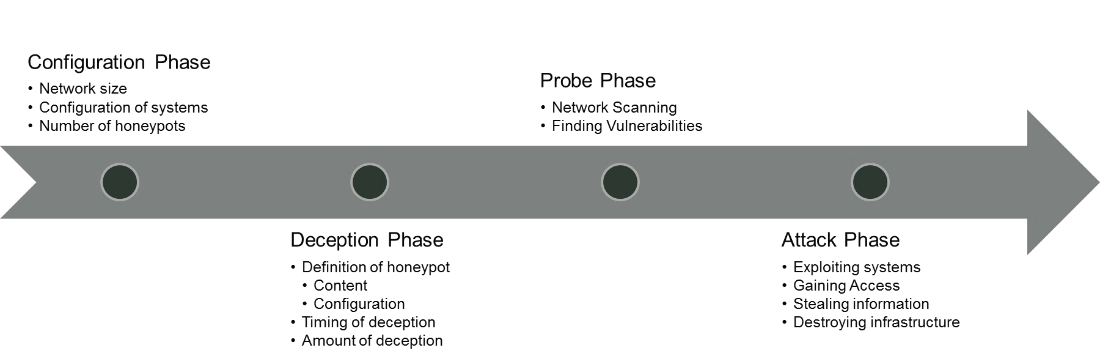
\includegraphics[scale=1.3]{Chap1/hacking.png}
  \caption{Hacking Phases}\label{fig:figure1}
\end{figure}      
\FloatBarrier
The \textit{probe phase} involves scanning of web-servers in the network for vulnerabilities; whereas, the \textit{attack phase} involves gaining access to different systems and stealing sensitive information or compromising the systems. The results of \textit{nmap} Figure \ref{fig:figure2} during the probing phase reveal which ports are currently open and which Operating system is running on the host. This information can be exploited by the hacker while choosing which type of system to attack or what vulnerability to exploit.
\FloatBarrier
\begin{figure}[!htbp]
\centering
  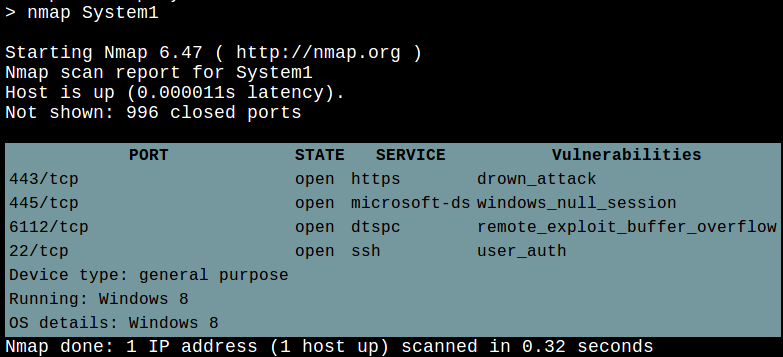
\includegraphics[scale=0.5]{Chap1/nmap.png}
  \caption{nmap Output}\label{fig:figure2}
\end{figure}      
\FloatBarrier

During the welcome phase, the table in Figure \ref{fig:figure3} is displayed to the hacker which shows the various operating system which is easy/difficult to attack along with services running on them. It is usually believed that UNIX based operating systems are less vulnerable to cyber attacks, compared to the older version of Windows. Due to a large number of open-source developers, it is likely that any flaws will be caught and fixed quickly. Thus, it is highly probable that hacker would attack the more vulnerable operating system in order to boost his chances to hack into the system. During the probe, participants performing as hackers could probe web-servers, some of which are honeypots. Once hackers probed the network, they could choose to attack any of the web-servers and try to copy the information to their system.
\FloatBarrier
\begin{figure}[!htbp]
\centering
  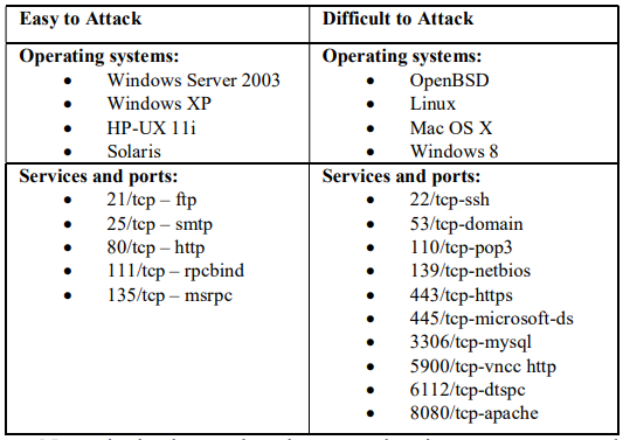
\includegraphics[scale=0.6]{Chap1/easy_diff.png}
  \caption{Operating Systems based on vulnerabilities}\label{fig:figure3}
\end{figure}
\FloatBarrier
\section{Literature Survey}
Aggarwal et al. \cite{Cyb02} proposed HackIT tool to bridge the gap between behavioral game-theory approaches and real-world cybersecurity tasks. HackIT tool provided features to create more specific set of actions and information needed for cyber-security tasks for both hackers and defenders. The paper discusses the use of HackIT tool to replicate the results of a laboratory experiment using a deception game. Results revealed that the average proportion of attacks was lower and not-attack actions were higher when deception occurred late in the game rather than earlier; and when the amount or deception was high compared to low [6]. This result was replicated in a real-world simulation tool called the HackIT.

In \cite{Cyb02}, the HackIT tool could be used for creating deception with limited number of systems only and for single player games only. It also describes the results from the experiment and discuss the implications of results for investigating the decision-making of hackers in the real world.

Achleitner et al. \cite{7971943} proposed a Reconnaissance deception network based on software defined networking to achieve deception by simulating virtual topologies. Their research\cite{7971943} describes various scanning techniques deployed by adversaries and how they fare against their RDS. Their system can simulate the topological as well as the physical characteristics of the network which deceives malicious network discovery by providing them with virtual information. Their system counters network reconnaissance by delaying scanning techniques of the adversaries and invalidating the collected information. They discuss the concept of virtual network views, based on a defined deception approach, to camouflage critical resources and place vulnerable endpoints at locations in a virtual network topology to significantly increase their detection time by an adversary. This provides us with a novel defense technique against malicious network reconnaissance which is required for targeted cyber attacks.
\section{Thesis Organisation}
This work is organised in 7 chapters.
\begin{itemize}
	\item Chapter~\ref{chap1_introduction} introduces the topic, providing a brief overview the background of the project and delves into the necessary literature. 
	\item Chapter~\ref{chap2} provides a brief overview about the working of the application and the features implemented in the project.
	\item Chapter~\ref{chap3} describes the experiment conducted using HackIT and discusses results and graphs obtained in detail. 
	\item Chapter~\ref{chap4} provides.
	\item Chapter~\ref{chap5} discusses.
	\item Chapter~\ref{chap6} discusses.
	\item Chapter~\ref{chap7} concludes the work and discusses future scope of the work.
	\item References are given in the bibliography.
\end{itemize}